\begin{frame}{Deux niveaux de blindage}
  \begin{figure}[h!tbp]
    \centering
    \subfigure[Niveau 1 de blindage]{\label{level1} 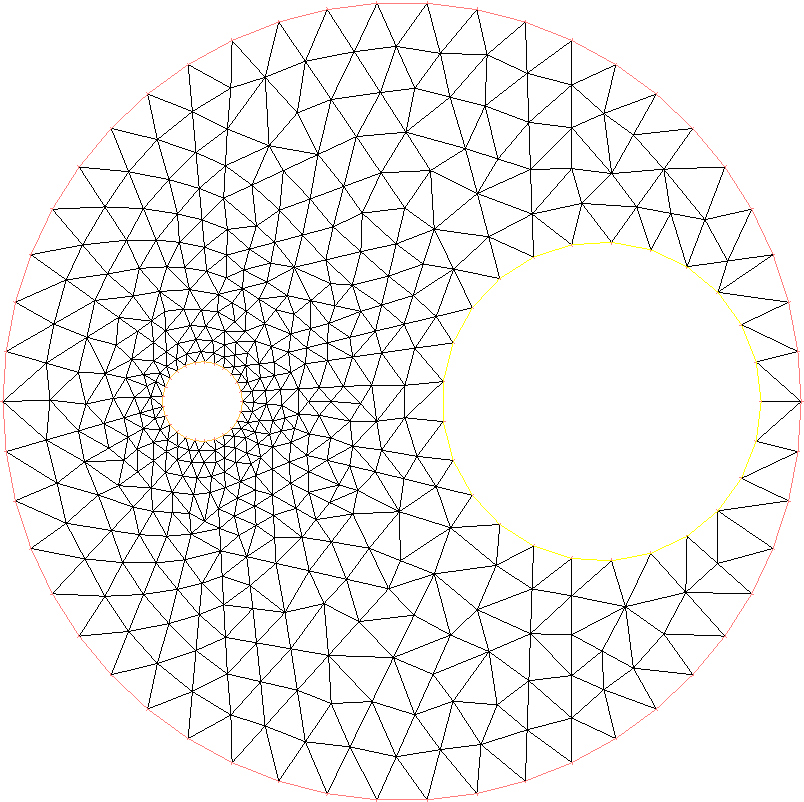
\includegraphics[width=.45\linewidth]{../figs/Th0.pdf}} \hspace{0.5cm}
    \subfigure[Niveau 2 de blindage]{\label{level2} 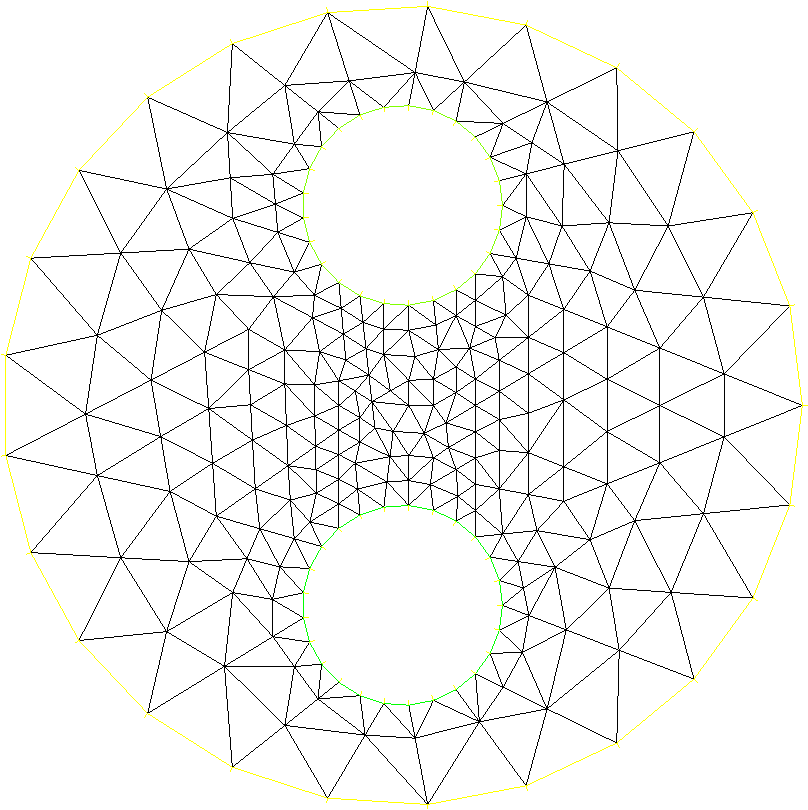
\includegraphics[width=.45\linewidth]{../figs/Th1.pdf}} %\hspace{0.75cm}
    %\subfigure[Trial basis functions in $P_2$]{\label{fig:trial:basis:functions} \includegraphics[width=0.3\linewidth]{basis_trial}}
    % \caption{Basis functions}
    \label{fig:basis:functions}
  \end{figure}
\end{frame}


\begin{itemize}
\item Résolution du problème \ref{eq:2} sur les maillages \ref{level1} et \ref{level2}
\item Assemblage de la matrice de conductivité $M$ présentée dans \ref{eq:3}
\item Calcul de la matrice d'inductance $L=M^{-1}$ présentée dans \ref{eq:4}
\item Vérification des propriétés de la matrice $L$
\end{itemize}

Calcul de la matrice d'inductance global

\Large

\[ L = P_I^T \left[ \begin{array} {cc}
L_{ext} &0 \\
0 & L_{int} \end{array}  \right] P_I , \qquad
P_I=
\left[ \begin{array} {cc}
1 & -\delta \\
0 & 1 \end{array}  \right]
 \]

avec $\delta$ la matrice de taille $N_{ext}\times N_{int}$ définie par

\normalsize
\begin{equation}
\delta(i,j)=
\begin{cases}
1 \qquad \text{si le conducteur $j+N_{ext}$ est dans le conducteur $i$,} \\
0 \qquad \text{sinon.}
\end{cases}
\end{equation}
